\documentclass[
% -- opções da classe memoir --
12pt,				% tamanho da fonte
%openright,			% capítulos começam em pág ímpar (insere página vazia caso preciso)
%openany,
twoside,			% para impressão em verso e anverso. Oposto a oneside
a4paper,			% tamanho do papel.
% -- opções da classe abntex2 --
%chapter=TITLE,		% títulos de capítulos convertidos em letras maiúsculas
%section=TITLE,		% títulos de seções convertidos em letras maiúsculas
%subsection=TITLE,	% títulos de subseções convertidos em letras maiúsculas
%subsubsection=TITLE,% títulos de subsubseções convertidos em letras maiúsculas
% -- opções do pacote babel --
english,			% idioma adicional para hifenização
brazil,				% o último idioma é o principal do documento
]{abntex2}

\usepackage[alf]{abntex2cite}	% Citações padrão ABNT

\usepackage{cmap}				% Mapear caracteres especiais no PDF
\usepackage{lmodern}			% Usa a fonte Latin Modern

\usepackage{amsthm}
\usepackage{amsmath}
\usepackage{amsfonts}
\usepackage{amssymb}
\usepackage{algpseudocode}
\usepackage{algorithm}

\usepackage{graphicx}			% Inclusão de gráficos
\usepackage{subcaption}

\usepackage[T1]{fontenc}		% Selecao de codigos de fonte.
\usepackage[utf8]{inputenc}		% Codificacao do documento (conversão automática dos acentos)

\addto\captionsbrazil{%
\def\bibname{References}%
}

\newtheorem{mydef}{Definição}
\newtheorem{myprop}{Proposição}

\addto\captionsbrazil{
  \renewcommand{\contentsname}%
    {Contents}%
}

\titulo{A Hybrid Heuristic for the Multi-objective Knapsack Problem}
\autor{Marcos Daniel V. Baroni}
\local{Vitória - Espírito Santo - Brasil}
\data{November 27, 2017}
\orientador[Advisor:]{Dr. Flávio Miguel Varejão}
%\coorientador{Equipe \abnTeX}
\instituicao{%
  Universidade Feredal do Espírito Santo -- UFES
  \par
  Departamento de Informática
  \par
  Programa de Pós-Graduação em Informática}
\tipotrabalho{Tese (Doutorado)}
% O preambulo deve conter o tipo do trabalho, o objetivo,
% o nome da instituição e a área de concentração
\preambulo{Tese de Doutorado apresentada de acordo
com o regimento do Programa de Pós-graduação
em Informática da Universidade
Federal do Espírito Santo.}

\makeindex


%%%%%%%%%%%%%%%%%%%%%%%%
% 1. Introdução:
%  (???) Motivação EDP
% 2. MOKP
%   2a. Algoritmos Exatos
%     - Bibliografia
%     - Bazgan's algoritmo
%   2b. Algoritmos Heurísticos
% 3. KDTree
%   3a. Use no Exato
%   3b. Uso no Heurístico
% 4. Experimentos
%   4a. KDT no Exato
%   4b. KDT no Heurístico
% 5. Conclusão
% A. Anexos: Experimentos EDP
%%%%%%%%%%%%%%%%%%%%%%%%

\begin{document}

%%%%%%%%%%%%%%%%%%%%%%%%
% Folhas               %
%%%%%%%%%%%%%%%%%%%%%%%%
\imprimircapa
\imprimirfolhaderosto*

\newcommand{\dtree}[1]{$#1$-d~tree}
\newcommand{\kdtree}{\dtree{k}}
\newcommand{\bsym}[1]{\boldsymbol{#1}}
%\newcommand{\sol}[1]{\boldsymbol{#1}}
\newcommand{\sol}[1]{#1}
\newcommand{\pnt}[1]{pnt(\sol{#1})}
\newcommand{\fsol}[1]{f(\sol{#1})}
\newcommand{\np}{m}
\newcommand{\nphard}{$\mathcal{NP}$-Hard}
\newcommand{\missingI}[1]{}
\newcommand{\missing}[1]{
  \begin{framed}
    {\scriptsize  #1}
  \end{framed}
}
\newcommand{\weight}[1]{w(\sol{#1})}
\newcommand{\obj}[2]{f_{#1}(\sol{#2})}
\newcommand{\bigweight}[1]{w\big(\sol{#1}\big)}
\newcommand{\setIN}{\{1, \ldots, n\}}
\newcommand{\ext}[2]{ext(\sol{#1}, \sol{#2})}
\newcommand{\domLess}[2]{ \sol{#1} \prec \sol{#2} }
%\newcommand{\logicAnd}{ \textrm{ and } }
\newcommand{\logicAnd}{ \land }
\newcommand{\logicOr}{ \lor}
\newcommand{\solSetA}{ Q }
\newcommand{\solSetB}{ R }
\newcommand{\solSett}{ S_* }
\newcommand{\solSet}{ S }
\newcommand{\rord}{\mathcal{O}_{rev}}
\newcommand{\cb}[2]{cb^{#1}(#2)}  % cost-benefit function
\renewcommand{\leq}{\leqslant}
\renewcommand{\geq}{\geqslant}
\newcommand{\floor}[1]{\left \lfloor{#1}\right \rfloor}

% bar graphs configs
\newcommand{\cmpH}{4.0cm}
\newcommand{\cmpW}{7cm}
\newcommand{\legX}{0.45}
\newcommand{\legY}{-0.30}
\newcommand{\scecore}{SCEcr }
\newcommand{\mokp}{MOKP}
\newcommand{\paretoset}{conjunto Pareto}
\newcommand{\paretosetII}{conjunto Pareto-ótimo}
\newcommand{\knapsackdominates}{domina segundo a mochila}

%%% Other Papers Defs Auxiliars %%%
%\newcommand{\dom}[2]{dom(#1, #2)}
\newcommand{\dom}{\underline{\Delta}}
\renewcommand{\ord}{\mathcal{O}}
%\newcommand{\domk}[2]{dom_k(#1, #2)}
\newcommand{\til}[1]{{#1'}}
\newcommand{\rel}{D}
\newcommand{\relk}{\rel_k}
\newcommand{\relki}[1]{\rel_k^{#1}}
\newcommand{\relkargs}[2]{\relk\big(#1, #2\big)}
\newcommand{\relkargsi}[3]{\relki{#1}\big(#2, #3\big)}
\newcommand{\nrel}{p}

\newcommand{\relI}{\rel_k^r}
\newcommand{\relII}{\rel_k^{\dom}}
\newcommand{\relIII}{\rel_k^{b}}

% big bullet
\newcommand{\bbt}{\,\begin{picture}(-1,1)(-1,-2)\circle*{5}\end{picture}\ }

\begin{folhadeaprovacao}

  \begin{center}
    {\ABNTEXchapterfont\large\imprimirautor}

    \vspace*{\fill}\vspace*{\fill}
    {\ABNTEXchapterfont\bfseries\Large\imprimirtitulo}
    \vspace*{\fill}
    
    \hspace{.45\textwidth}
    \begin{minipage}{.5\textwidth}
        \imprimirpreambulo
    \end{minipage}%
    \vspace*{\fill}
   \end{center}
    
   Work approved. \imprimirlocal, November 27, 2017:

   \assinatura{\textbf{\imprimirorientador} \\ Advisor} 
   \assinatura{\textbf{Dr.ª Simone de Lima Martins} \\ Guest}
   \assinatura{\textbf{Dr. Arlindo Gomes de Alvarenga} \\ Guest}
   %\assinatura{\textbf{Professor} \\ Convidado 3}
   %\assinatura{\textbf{Professor} \\ Convidado 4}
      
   \begin{center}
    \vspace*{0.5cm}
    {\large\imprimirlocal}
    \par
    {\large\imprimirdata}
    \vspace*{1cm}
  \end{center}
  
\end{folhadeaprovacao}


\begin{resumo}
Resumo...
\vspace{\onelineskip}

\noindent
\textbf{Palavras Chave}:
Multi-objective Knapsack Problem,
Metaheuristic,
Shuffled Complex Evolution,
Multi-dimensional indexing
\end{resumo}

\begin{resumo}[Abstract]
 \begin{otherlanguage*}{english}
Many real applications like project selection, capital budgeting and cutting stock involves optimizing multiple objectives that are usually conflicting and can be modelled as a multi-objective knapsack problem (MOKP).
Unlike the single-objective case, the MOKP is considered a NP-Hard problem with
considerable intractability.
This work propose a hybrid heuristic for the MOKP based on the
shuffled complex evolution algorithm.
A multi-dimensional indexing strategy for handling large amount of intermediate
solutions are proposed as an optimization, which yields considerable
efficiency, especially on cases with more than two objectives.
A series of computational experiments show the applicability of the proposal
to several types of instances.

\noindent
\textbf{Keywords}:
Multi-objective Knapsack Problem,
Metaheuristic,
Shuffled Complex Evolution,
Multi-dimensional indexing
\end{otherlanguage*}
\end{resumo}

% Falar brevemente sobre o MOKP
% Falar brevemente sore a estratégia de indexação
% Resumir os resultados obtidos

\missingt{
Observar as 5 regras:\\
1. A general statement introduciong the broad reserach area of the particular topic being investigated;\\
2. An explanation of the specific problem (difficulty, obstavle, challange) to be solved;\\
3. A review of existing or standard solutions to this problem and their limitations;\\
4. An outline of the proposed new solution;\\
5. A summary of how the solution was evaluated and what the outcomes of the evaluation were.
}



%%%%%%%%%%%%%%%%%%%%%%%%
%  Sumário             %
%%%%%%%%%%%%%%%%%%%%%%%%
\pdfbookmark[0]{\contentsname}{toc}
\tableofcontents*

%%%%%%%%%%%%%%%%%%%%%%%%
%  Texto               %
%%%%%%%%%%%%%%%%%%%%%%%%
% Introdução
\chapter{Introdução}

% MO problems
\begin{frame}
\frametitle{Multi-objective problems}
\textbf{Multi-objective problems} are optimization problems involving optimizing multiple criteria.
\pause
\begin{itemize}
  \item{ Usually conflicting criterias; }\pause
  \item{ A set of \textit{optimal} (non-dominated) solutions; } \pause
  \item{ Models many real applications. }
\end{itemize}
\vfill
\end{frame}

% MOKP
\begin{frame}
\frametitle{The multi-dimensional knapsack problem}
The \textbf{multi-dimensional knapsack problem} (MOKP)
is one of the most important multi-objective problems.
\pause
\begin{itemize}
  \item{ Is a generalization of the $0-1$ knapsack problem (\nphard); }\pause
  \item{ Models project selection, capital budgeting, cargo loading, flow shop scheduling and others;} \pause
  \item{ Models many real applications; }
\end{itemize}
\end{frame}

% Motivation
\begin{frame}
\frametitle{Motivation}
Several exact approaches have been proposed in the literature for
solving the MOKP. \\ \pause
\vfill
However no effective exact method for large MOKP, expecially with
more than two objectives. \\ \pause
\vfill
Even for the bi-objective case, some medium sized instances
has shown to be hard to solve exactly. \\ \pause
\vfill
This reason motivates the development of heuristic methods.
\vfill
\end{frame}

% The Proposal
\begin{frame}
\frametitle{Proposal}
This work proposes the development of a heuristic for the MOKP
based on an evolutionary algorithm called shuffled complex evolution (SCE).
\\ \medskip \pause
As a performance improvement for the approach,
a multi-dimensional indexing strategy
will be used for handling the large amount of solutions.
\\ \medskip \pause
The SCE has been successfully used for solving optimization problems, among then,
the multi-dimensional knapsack problem (MKP) (also a contribution of this work).
\end{frame}

% Contributions and Publications
\begin{frame}
\frametitle{Contributions and Publications}\pause
\begin{enumerate}
\item{
\textbf{Efficient indexing strategy for MOKP solutions:} \pause
\begin{itemize}
 \item[{\tiny$\bullet$}] { BARONI, M. D. V; VAREJ\~AO, F. M. Multi-dimensional indexing on dynamic programming for multi-objective knapsack problem. \textit{International Transactions in Operational Research}, Wiley Online Library, 2017, Submitted. }
\end{itemize}
} \pause
\medskip
\item{
\textbf{A SCE algorithm for the MKP:} \pause
\begin{itemize}
  \item[{\tiny$\bullet$}] { BARONI, M. D. V; VAREJ\~AO, F. M. A shuffled complex evolution algorithm
  for the multidimensional knapsack problem. In: \textit{Progress in Pattern Recognition, Image Analysis, Computer Vision, and Applications.} [S.l.]: Springer, 2015. p. 768-775. }
  \pause
 \item[{\tiny$\bullet$}] { BARONI, M. D. V; VAREJ\~AO, F. M. A shuffled complex evolution algorithm
  for the multidimensional knapsack problem using core concept. In: IEEE. \textit{Evolutionary Computation (CEC), 2016 IEEE Congress on.} [S.l.], 2016 p. 2718-2723. }
\end{itemize}
} \pause
\medskip
\item{
\textbf{Hybrid heuristic for MOKP:} \pause
\begin{itemize}
 \item[{\tiny$\bullet$}] { BARONI, M. D. V; VAREJ\~AO, F. M. An efficient shuffled complex evolution algorithm for the multi-objective knapsack problem. In: IEEE \textit{Evolutionary Computation (CEC), 2018 IEEE Congress on.} [S.l.], 2018, In Preparation }
\end{itemize}
}
\end{enumerate}
\end{frame}


% Multi-objective Knapsack Problem
\chapter{O Problema da Mochila Multi-objetivo}

%%% Definição de problema multi-objectivo

Em problemas reais é comum a existência de situações em que deseja-se otimizar
mais de um objetivo os quais, geralmente, são conflitantes.
Estes problemas são chamados multiobjetivos e tipicamente não possuem
uma solução sendo a melhor em todos os objetivos, mas as possuem várias
soluções de interesse chamadas \emph{soluções eficientes}.

Um problema de otimização multi-objetivo com $\np$ objetivos pode ser descrito como uma
função vetorial $f(x) = \big(f_1(x), \ldots, f_p(x)\big)$
para a qual deseja-se encontrar um vetor $x \in X$
que maximize simultaneamente as $\np$ funções objetivo.
Formalmente:
\begin{align*}
  \text{max} ~ f(x) &=
    \big(f_1(x)
    ,f_2(x)
    ,\ldots
    ,f_{\np}(x)\big) \\
  \text{sujeito a} ~ x & \in X
\end{align*}

\begin{mydef}[Dominância, Eficiência e \paretoset]
Considere um problema de otimização multi-objetivo.
Diz-se que uma solução $x \in X$
\emph{domina} uma solução $y \in X$, denotado por $\text{dom}(x, y)$
se, e somente se, $x$ é ao menos tão boa quanto
$y$ em todos os objetivos e melhor que $y$ em ao menos um dos objetivos.
Formalmente:
\begin{displaymath}
    \text{dom}(x, y) = \left\{
      \begin{array}{l}
          \forall i \in \{1, 2, \ldots, \np\}: f_i(x) \geq f_i(y) ~\text{e}\\
          \exists j \in \{1, 2, \ldots, \np\}: f_j(x) > f_j(y)
  \end{array} \right.
\end{displaymath}
Uma solução $x \in X$ é dita \emph{eficiente}, denotado por $\text{eff}(x)$,
se, e somente se, $x$ não é dominada por nenhuma outra solução pertencente a $X$.
Formalmente:
\begin{displaymath}
  eff(x) \iff \nexists \big(y \in X \wedge dom(y, x) \big)
\end{displaymath}
O conjunto de todas as soluções eficientes de um problema multi-objetivo,
denotado por $Par(X)$, é chamado de \emph{\paretoset{}} ou \emph{\paretosetII{}}.
Formalmente:
\begin{displaymath}
  Par(X) = \{ x \in X \;|\; \text{eff}(x)\}
\end{displaymath}
\end{mydef}

Resolver um problema multi-objetivo consiste em determinar seu \paretoset{}.
Este conceito foi primeiramente elaborado por Vilfredo Pareto em 1896, que
enunciou a relação Pareto-Ótima que diz: ``não é possível melhorar uma característica
do problema sem piorar outra'', o que caracteriza a relação conflitante entre os
objetivos na otimização multi-objetivo.

Na Figura~\ref{fig:dom-def} ilustra o conceito de dominância.
A solução marcada domina todas as soluções existentes na área hachurada.
As soluções em destacadas na Figura~\ref{fig:eff-def} formam um \paretoset por
dominarem sobre todas as outras soluções.

\begin{figure}
    \centering
    \begin{subfigure}[t]{0.3\textwidth}
        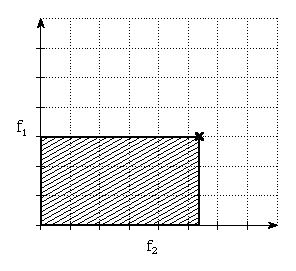
\includegraphics[width=\textwidth]{img/mokp/dom-def}
        \caption{Região de dominância de uma solução.}
        \label{fig:dom-def}
    \end{subfigure}
    \qquad
    \begin{subfigure}[t]{0.3\textwidth}
        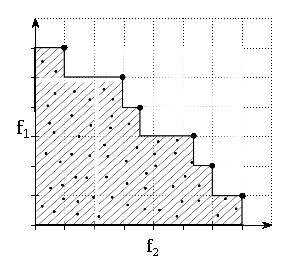
\includegraphics[width=\textwidth]{img/mokp/pareto-def}
        \caption{Exemplo de \paretoset.}
        \label{fig:eff-def}
    \end{subfigure}
    \caption{Exemplos de solução dominante e \paretoset.}
    \label{fig:mo-defs}
\end{figure}

%%% Intro ao MOKP

Um dos problemas multiobjetivos mais importantes da literatura
é o problema da mochila multiobjetivo (\mokp{}).
Muitas problemas reais podem ser modelados como uma instância do \mokp{}
como seleção de projetos~\cite{teng1996multiobjective},
orçamento de capital~\cite{rosenblatt1989generating},
carregamento de carga~\cite{teng1996multiobjective}
e planejamento de estoque~\cite{ishibuchi2015behavior}.

\missing{Comentar sobre a dificuldade de problemas MObj.
Exploão do pareto com o aumento da quantidade de objectivos.
Poucos métodos extados eficientes, geralmente utiliza-se métodos heurísticos.}

%%%%%%%%%%%%%%%%%%%%%%%%%
%%% Definição do MOKP %%%
%%%%%%%%%%%%%%%%%%%%%%%%%
O problema da mochila multi-objetivo pode ser descrito como uma função vetorial
$f$ que mapeia uma variável de decisão (solução) a uma tupla de $\np$ valores
(objetivos).
Formalmente:
\begin{align*}
  \text{max} ~ \sol{y} &= f(\sol{x}) =
    \big(f_1(\sol{x})
    ,f_2(\sol{x})
    ,\ldots
    ,f_{\np}(\sol{x})\big) \\
  \text{sujeito a} ~ \sol{x} & \in X
\end{align*}
onde $\sol{x}$ é a \emph{variável de decisão}, $X$ denota o conjunto de
soluções viáveis e $\sol{y}$ representa o \emph{vetor de objetivos} para os quais
deseja-se maximizar.

Vale resaltar que o tamanho do \paretoset para o problema em questão
tende a crescer rapidamente com o tamanho do problema, especialmente com o
número de objetivos.

Uma instância de um problema da mochila multi-objetivo (\mokp{}) com $\np$
objetivos consiste em uma capacidade inteira $W >0$ e $n$ itens.
Cada item $i$ possui um peso inteiro positivo $w_i$ e $\np$ lucros inteiros
$p_i^1, p_i^2, \ldots, p_{i}^{\np}$ não negativos.
O lucro $p_i^k$ representa a contribuição do $i$-ésimo item
para com o $k$-ésimo objetivo.
Uma solução é representada por um conjunto $\sol{x} \subseteq \{1, \ldots, n\}$
contendo os índices dos itens incluídos na mochila.
Uma solução é viável se o peso total incluído na mochila não ultrapassa
a capacidade da mochila.
Formalmente a definição do problema é a seguinte:
\begin{align*}
  \text{max   } & f(x) =
    \big(f_1(x) ,f_2(x) ,\ldots ,f_{\np}(x)\big) \\
  \text{subject to   } & w(x) \leq W \\
  & x \in \{0, 1\}^n\\
  \text{where} \phantom{mmmmm} \\
  %I_n &= \{1, \ldots, n\}\\
  f_j(x) &= \sum_{i = 1}^n p^j_i x_i \quad j = 1, \ldots, \np\\
  w(x) &= \sum_{i = 1}^n w_i x_i
\end{align*}

O \mokp{} é considerado um problema \nphard{} visto set uma generalização
do bem conhecido problema da mochila $0-1$, para o qual $\np = 1$.
É consideravelmente difícil determinar o \paretoset para um \mokp{},
especialmente para vários objetivos.
Até mesmo para casos bi-objetivos, problemas pequenos podem se apresentar
intratáveis.
Por este motivo interessa-se no desenvolvimento de métodos eficientes
para manipular uma grande quantidade de soluções, o que pode eventualmente
trazer tratabilidade a instâncias antes intratáveis.

A literatura contém várias propostas para resolver o \mokp{} de forma exata.
Porém, nenhum método tem provado ser eficiente para grande instâncias
com mais de dois objetivos.
Mesmo para problemas bi-objetivo, algumas instâncias de tamanho considerado
médio têm aprestando difculdades na determinação da solução exata, o que
tem motivado o desenvolvimento de métodos heurísticas que buscam determinar
um \paretoset aproximado em tempo computacional razoável.

\section{Métodos Exatos}
O algoritmo de Nemhauser e Ullmann é um algorimto de programação dinâmica
que resolve problemas da mochila de forma genérica aplicando o conceito de
dominância da mochila para remover soluções parciais que não resultarão em
soluções eficientes, ou seja, soluções que irão compor o \paretoset (conjunto solução).

\begin{algorithm}
  \caption{O algoritmo de Nemhauser e Ullmann para o \mokp.}
  \label{alg:nemull}
  \Kw{$\bsym{p}, \bsym{w}, W$}
\Begin{
  \SetAlgoLined
  $S^0 = \big\{\emptyset\big\}$\;
  \For{$k \gets 1, n$}{
    $S_*^k = S^{k-1} \cup \{\sol{x} \cup k \:|\: \sol{x} \in S^{k-1}\}$\;
    TODO...\;
  }
  $P = \{\sol{x} \:|\: \nexists \sol{a} \in S^n: \dom{a}{x} \;|\; \weight{x} \leq W \}$\;
  \textbf{return} $P$\;
}
\end{algorithm}

O algoritmo inicia definindo uma solução inicial $S^0$ contendo apenas a solução
vazia (linha 2).
Na $k$-ésimo iteração o algoritmo recebe um conjunto $S^{k-1}$ contendo
soluções exclusivamente compostas pelos primeiros ${k-1}$ itens,
ou seja, $\forall\sol{x} \in S^{k-1}, \sol{x} \subseteq \{1, \ldots, k-1\}$.
O conjunto $S^{k-1}$ é então expandido adicionando-se uma cópia de cada uma
das suas soluções mas desta vez incluindo o $k$-ésimo item (linha 4),
formando o conjunto $S^k_*$, o qual possui o dobro da cardinalidade de $S^{k-1}$.
O conjunto $S^k_*$..

Apesar de sua simplicidade o Algoritmo~\ref{alg:nemull} é consideravelmente poderoso.
Contudo o potencial crescimento exponencial do \paretoset para o \mokp
compromete severamente o seu desempenho.
Uma forma de atacar este problema é tentar reduzir ainda mais a quantidade de
soluções parciais manuseadas durante as iterações do algoritmo.
Três propostas...

\section{Métodos Heurísticos}
\section{Evolução estocástica por complexos}

O Algoritmo de Evolução estocástica por complexos (EEC),
\emph{Shuffled Complex Evolution} em inglês,
é um algoritmo evolutivo populacional proposto por Duan~\cite{duan1992effective}
e tem sido utilizado com sucesso em problemas de escalonamento
\cite{zhao2015shuffled}, seleção de projetos~\cite{elbeltagi2007modified},
problema da mochila $0-1$~\cite{bhattacharjee2014shuffled} e
problema da mochila multi-dimensional~\cite{baroni2015shuffled,baroni2016shuffled}.

O EEC é inspirado na evolução natural que ocorre de forma simultânea em
comunidades independentes.
O algoritmo trabalha com uma população particionada em $N$ comunidades,
ou complexos, cada uma contendo $M$ indivíduos.
Inicialmente a população de $N*M$ indivíduos é tomada aleatoriamente do espaço
de soluções viáveis.
Após esta inicialização a população é ordenada em ordem descrecente de aptidão
e o melhor global é identificado.
Toda a população é então particionada em $N$ complexos, cada um contendo $M$ indivíduos.
Neste processo de distribuição aleatória o primeiro indivíduo é incluído
no primeiro complexo, o segundo indivíduo no segundo complexo, o $M$-ésimo
indivíduo no $M$-ésimo complexo, o $M+1$-ésimo indivíduo no primeiro complexo,
e assim por diante.

O próximo passo após a distribuição dos indivíuos em complexos é evoluir cada
complexo uma quantidade constante $K'$.
Neste processo, considerando que os indivíduos em cada complexo estão ordenados
em ordem decrescente de aptidão, um subcomplexo é de $P$ indivíduos é selecionado
dentre o complexo utilizando uma distribuição triangular, em que o $i$-ésimo
indivíduo tem a probabilidade $p_i = \frac{2(n+1-i)}{n(n+1)}$ de ser selecionado.
A utilização da distribuição triangular tem por objetivo priorizar os indivíduos
com melhor aptidão, favorecendo assim a convergência do algoritmo.

Após a seleção do subcomplexo, o seu pior indivíduo é identificado para ser
subtituido por um novo indivíduo.
Este novo indivíduo é gerado através do cruzamento do pior indivíduo e um outro
indivíduo com melhor aptidão.
Primeiramente o melhor indivíduo do subcomplexo é considerado.
Caso o indivíduo gerado não seja melhor que o pior indivíduo selecionado,
o melhor indivíduo do complexo é então usado no cruzamento.
Se este último cruzamento não resultou em melhoria, o melhor indivíduo de toda
a população é considerado.
Finalmente, se todos os cruzamentos não foram capaz de gerar um melhor indivíduo,
esta pior solução selecionada é substituída por um novo indivíduo retirado de
forma aleatória do espaço de soluções viáveis.
Este último procedimento é importante para impedir que o algoritmo fique
\emph{preso} num ótimo local.
A Figura~\ref{img:flow2} apresenta o procedimento de evolução descrito acima
em um fluxograma.

\begin{figure}[]
  \centering
  \begin{minipage}[b]{0.42\textwidth}
    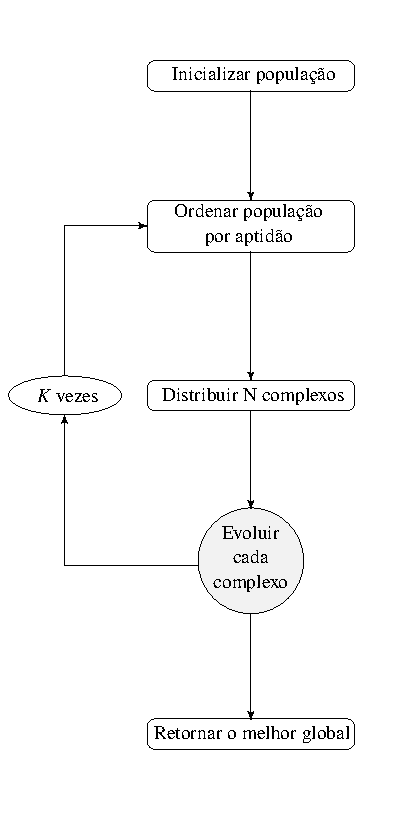
\includegraphics[width=\textwidth]{img/sce/flow1}
    \caption{The shuffled complex evolution algorithm.}
    \label{img:flow1}
  \end{minipage}
  \hfill
  \begin{minipage}[b]{0.42\textwidth}
    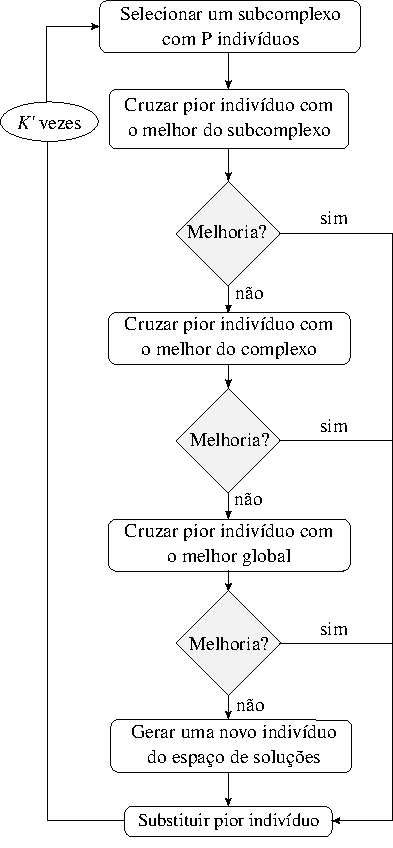
\includegraphics[width=\textwidth]{img/sce/flow2}
    \caption{The evolving stage of SCE for a single complex.}
    \label{img:flow2}
  \end{minipage}
\end{figure}

Após evoluir todos os $N$ complexos toda a população é novamente ordenada
em ordem descrecente de aptidão e o processo continua até que a condição
de parada seja satisfeita.

A Figura~\ref{img:flow1} apresenta os passos do algoritmo ECC num fluxograma
em que a condição de parada é a execução de uma quantidade fixa de $K$ evoluções.


\section{O EEC para o MOKP}
Como pode-se notar em sua descrição, o EEC é facilmente aplicável a qualquer
problema de otimização, inclusive o MOKP, desde que seja possível (a) definir
um procedimento de criação de uma nova solução alteatória viável e (b) definir
um procedimento de cruzamento entre duas soluções.
Esses dois procedimentos para o MOKP são descritos no Algoritmo~\ref{alg:new}
e Algoritmo~\ref{alg:cross}.

\begin{algorithm}
  \begin{algorithmic}[1]
    \Procedure{Nova solução aleatória}{}
      \State $v \leftarrow $ shuffle($1, 2, \ldots, n$);
  	\State $s \leftarrow \vec{0}$; \Comment{solução vazia}
      \For{$ i \leftarrow 1:n$ }
  	  \State $s[v_i] \leftarrow 1$; \Comment{inserção de item}
  	  \If{ $w(s) > W$ } \Comment{verificação de viabilidade}
  	    \State $s[v_i] \leftarrow 0$;
        \EndIf
  	\EndFor
    \State retorna $s$
    \EndProcedure
  \end{algorithmic}
  \caption{Geração de uma nova solução para o MOKP.}
  \label{alg:new}
\end{algorithm}

Para se contruir uma nova solução aleatória para o MOKP (Algoritmo~\ref{alg:new})
os índices dos $n$ itens são primeiramente permutados em ordem aleatória e
armazenados em uma lista $v$ (linha 2).
Uma nova solução vazia é definida (linha 3).
O algoritmo tenta de forma iterativa preencher a solução com um item retirado
da lista de índices (linhas 4-9).
A viabilidade da solução é então verificada: se o item inserido tornar a solução
inviável (linha 6) ele é então retirado da solução (linha 7).
Após testar a inserção de todos os itens a solução contruida é retornada.

\begin{algorithm}
\begin{algorithmic}[1]
  \Procedure{Cruzamento}{$s:$ pior indivíduo, $b:$ melhor indivíduo, $c$}
    \State $v \leftarrow $ shuffle($1, 2, \ldots, n$);
    \For{$ i \leftarrow 1:c$ };
	  \State $s[v_i] \leftarrow b[v_i]$; \Comment{carregamento do gene}
	\EndFor
	\If{$w(s) > W$}
	  \State reparar $s$;
	\EndIf
	\State computar aptidão de $s$;
  \State retornar $s$;
  \EndProcedure
\end{algorithmic}
\caption{Procedimento de cruzamento de duas soluções para o MOKP.}
\label{alg:cross}
\end{algorithm}

O procedimento de cruzamento (Figura~\ref{alg:cross}) recebe como entrada
$s$ o pior indivíduo vindo do subcomplexo selecionado, $b$ um indivíduo com
maior aptidão que $s$ e parâmetro $c$ sendo o número de genes a serem carregados de $b$.
O parâmetro $c$ controla o quão similar o novo indivíduo será do melhor indivíduo
dado como entrada.
Primeiramente os índices dos $n$ itens são permutados em uma ordem aleatória e armazenados numa lista
(linha 2).
Os $c$ genes escolhidos aleatoriamente é então carregado do melhor indivíduo para
o pior indivíduo (linhas 3-5).
Em seguida a viabilidade da solução é verificada (linha 6) e então reparada
se necessário (linha 7).
Finalmente a aptidão da solução gerada é atualizada (linha 9) e então retornada (linha 10).


% KD-tree
\chapter{A k-d tree}
% Falar sobre a utilização de estrutura de dados.

\section{Verificação de dominância e a busca de faixa}

Como dito anteriormente, solucionar um problema multi-objetivo significa
apresentar o seu \paretoset{}, ou seja, o conjunto de soluções não dominadas.
Geralmente o processo de solução compreende-se em contruir este conjunto de
soluções de forma incremental.
Por este motivo, um dos procedimentos mais executados durante o processo é
verificar se uma determinada solução é dominada por alguma outra solução
existente num conjunto candidato.
Um algoritmo pode até mesmo necessitar de extrair um cojunto cobertura, ou seja,
extrair todas as soluções não-dominadas de um grande conjuto de soluções.

Esta operação deve demandar exforço quadrático sobre o número total de soluções
se implementada como uma comparação par-a-par.
Entretanto, se as soluções forem interpretadas como pontos em um espaço
multi-dimensional, podemos deduzir da Equação~\ref{eq:dom} que esta operação
corresponde em verificar a existência um ponto numa determinada região
do espaço. O mesmo pode ser considerado no caso mais específico para a dominância
da mochila, segundo a Equação~???.
Formalmente:
\begin{align*}
    & x \dom y \; \Longleftrightarrow \; \pnt{y} \in R(\sol{x}) \\
  \text{where} \phantom{mmmmm} \\
    \pnt{x} &= \big(\obj{1}{x}, \ldots, \obj{\np}{x}, \weight{x}\big) \\
    R(\sol{x}) &= \left\{ a \in \mathbb{R}^{\np+1} \;\middle|\;
      a_{\np+1} \leq \weight{x}
      \, \text{ and } \,
      a_i \geq \obj{i}{x}, \; i \in \{1, \ldots, \np\}
      \right\}
\end{align*}

\missing{Colocar referência para a equação de dominância da mochila (texto acima).}

O problema de determinar a existência de um ponto numa determinada região do
espaço é já bem conhecido da computação e chama-se problema da
\emph{busca de baixa} (ou \emph{range search} em ingês)~\cite{agarwal1999geometric}.
O problema de busca de faixa é largamente aplicado, por exemplo, na área da
computação gráfica e jogos, onde é necessário se verificar a colisão entre pontos e polígonos.
Para se ter uma solução eficiente deste problema evitando o esforço computacional
quadrático, os pontos devem ser indexados multidimensional.....
\missing{Melhorar parágrafo acima e conferir texto inicial do parágrafo abaixo.}

Devido a sua simplicidade e eficiência, a estrutura de dados mais utilizada
para o problema é a \emph{\kdtree}~\cite{preparata2012computational}.
Proposta por Jon Louis Bentley em 1957~\cite{bentley1975}, a \kdtree{} é um tipo de
árvore binária de construção simples e baixa utilização de memória.
Apesar de sua simplicidade, além da operação de buca de faixa, a \kdtree{}
suporta outras operações como busca de vizinho mais próximo.
Por este motivo é também bastante utilizada em algoritmos de
clasterização~\cite{kanungo2002efficient, indyk1998approximate}
e renderização gráfica~\cite{owens2007survey}.

Como uma árvore binária comum, a cada nível recursivo da árvore
a \kdtree{} subdivide os dados em duas partes.
Porém, diferentemente de uma árvore de busca binária comum, as quais utilizam
apenas uma \emph{chave} em todos os níveis da árvore, a \kdtree{} utiliza um
total de $k$ chaves fazendo um revezamento circular entre as chaves à medida
que caminha nos níveis da árvore.

A Figura~\ref{fig:kdom-kd} apresenta (a) um conjunto de pontos dispostos num
espaço bi-dimensional e indexados por uma (b) \dtree{2}.
O primeiro e terceiro nível da \dtree{2} indexa a componente $x$ dos pontos,
enquanto o segundo nível indexa a componente $y$.
Cada ponto indexado pela árvore subdivide o espaço em dois de acordo
com o valor da componente que está sendo indexada.
A subdivisão do espaço é representada na figura por uma linha mais grossa.

\begin{figure}
  \centering
  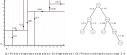
\includegraphics[scale=4.8]{img/kdt/dom-kd}
  \caption{Exemplo de pontos indexados por uma \kdtree{}.}
  \label{fig:kdom-kd}
\end{figure}

A Figura~\ref{fig:query} apresenta um exemplo de operação de verificação de
dominância utilizando uma \dtree{2} como estrutura de indexação.
A área acinzentada não tem intersecção com a área dominada pelo ponto $x$
(área hachurada), portanto as soluções dentro da área acinzentada não são
avaliadas.

\missing{Propor passo-a-passo da operação.}

\begin{figure}
  \centering
  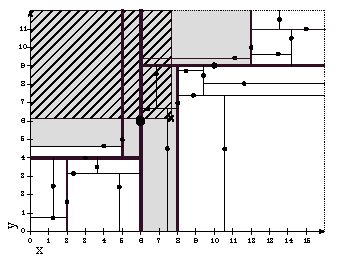
\includegraphics[scale=1.7]{img/kdt/query}
  \caption{Exemplo de operação de verificação de dominância utilizando a \kdtree{}.}
  \label{fig:query}
\end{figure}

Com relação à eficiência da \kdtree{} é importante considerar que não é
recomendável escalar de forma arbitrária o número $k$ de dimensões
indexadas pela \kdtree{}, esperando assim escalar também sua eficiência.
Mesmo que o dado possua todas estas dimensões.
Como regra geral considera-se que um \kdtree{} é adequada para indexar um
conjunto com $n$ pontos se $n$ não for muito maior que $2^k$\cite{toth2004handbook},
caso contrário, a performance da \kdtree{} se assemelhará a de uma busca
linear exaustiva.

Espera-se que a \kdtree{} auxilie as operações de verificação de dominância
\emph{podando} uma grande quantidade de soluções, demandando um menor número
de comparações entre soluções, melhorando assim a performance dos algoritmos.

% Falar um pouco sobre arvore binária.

% Definir a árvore kdtree


% Experimentos
\chapter{Experimentos}
Experimentos computacionais foram realizados com o objetivo de avaliar a
aplicação da proposta de indexação multidimensional ao MOKP,
através da observação do número de avaliações de solução e do tempo computacional.
Os testes foram divididos em dois grupos visando o contexto
exato e o heurístico respectivamente.
Em ambos os grupos a performance dos algoritmos utilizando a
indexação proposta pela literatura foi comparada à performance utilizando a
indexação multidimensional proposta por este trabalho.

Para o primeiro grupo, que visa analisar a aplicação da proposta no contexto exato,
foi utilizado o algoritmo Bazgan, por ser considerado pela literatura atual como
o algoritmo exato mais eficiente para o MOKP.
As instâncias consideradas neste primeiro grupo foram baseadas nas mesmas
utilizadas pela literatura em \emph{benchmarks} de algoritmos exatos~\cite{bazgan2009, figueira2013algorithmic, correia2018}.

Para o segundo grupo de experimentos, visando analisar a aplicação da proposta
no contexto heurístico, foi utilizada a implementação do SCE para o MOKP, proposta neste trabalho.
Neste segundo grupo, foram consideradas as instâncias utilizadas
pela literatura para \emph{benchmarks} de heurísticas para o MOKP~\cite{zitzler1998multiobjective,zitzler2001spea2, deb2002fast, zhang2007moea, zouache2018cooperative}.

Ambos os conjuntos são compostos por instâncias de 2 e 3 objetivos.
Ambos os algoritmos foram implementados na linguagem C e testados em
máquinas Intel\textsuperscript{\textregistered} Core\textsuperscript{TM} i5-3570 3.40HGz
com 4Gb de RAM com sistema operacional Linux versão 3.19.0 compilados utilizando
GCC versão 7.3.1 com parâmetro de otimização -O3.

\section{Contexto Exato - Algoritmo Bazgan}

Para o contexto exato, este trabalho não utilizou exatamente as mesmas instâncias utilizadas
pelos autores originais por estas não terem sido divulgadas.
As instâncias foram então novamente geradas aleatoriamente seguindo as mesmas regras de
distribuição definidas no trabalho original.

\missingf{Retirei: "Os autores originais foram contactados em seus e-mail porém não houve resposta.". Não fica bem escrever isso 
no texto. Se for questionado, fala oralmente na defesa.

\resp Ok.

}

As instâncias bi-objetivo são divididas em 4 tipos:
\begin{enumerate}
  \item[A)] Aleatórias: $
    p^j_i \in [1, 1000],
    w_i \in [1,1000]$.
  \item[B)] Não-conflitantes: $
    p^1_i \in [111, 1000],\\
    p^2_i \in [p^1_i - 100, p^1_i + 100],\\
    w_i \in [1,1000]$.
  \item[C)] Conflitantes: $
    p^1_i \in [1, 1000],\\
    p^2_i \in [max\{900-p^1_i;1\}, min\{1100-p^1_i, 1000\}],\\
    w_i \in [1,1000]$.
  \item[D)] Conflitantes com pesos correlacionados: $
    p^1_i \in [1, 1000],\\
    p^2_i \in [max\{900-p^1_i;1\}, min\{1100-p^1_i, 1000\}],\\
    w_i \in [p^1_i+p^2_i-200, p^1_i+p^2_i+200]$.
\end{enumerate}
onde $\in [a,b]$ denota uma distribuição uniforme aleatória no intervalo $[a,b]$.
Para todas as instâncias foi atribuído $W=\frac{1}{2}\floor{\sum^n_{k=1} w^k}$.
Para cada tipo e valor de $n$ foram geradas dez instâncias.
Os valores de $n$ utilizados em cada tipo estão descritos na Tabela~\ref{tab:cpu2dim}.
O termo ``conflitante'' refere-se aos valores de $p^j_i$ em cada item:
em instâncias conflitantes, itens com altos valores de $p^1$ tendem a ter
baixos valores de $p^2$ enquanto que itens com baixos valores de $p^1$ tendem a ter
altos valores de $p^2$.
Por sua vez, instâncias não-conflitantes possuem itens cujos valores de $p^j_i$ não possuem
relação com o peso $w_i$,

Devido a este caráter não-conflitante, instâncias do tipo B
tendem a possuir itens com valores de eficiência bastante discrepantes entre si.
Essa discrepância acaba reduzindo a combinação de itens geradores de soluções eficientes,
resultando em conjuntos Pareto de tamanho reduzido.
Por este motivo, as instâncias do tipo B são consideradas mais fáceis.

O aspecto conflitante das instâncias do tipo $D$, por sua vez, dificulta a decisão
de quais itens são mais eficientes que outros, resultando em
muitas boas combinações de solução e, consequentemente, em \paretoset{} aumentados.
Diante disso, as instâncias do tipo $D$ são consideradas mais difíceis.

Para os experimentos com $3$-objetivo considerou-se
a generalização introduzida por~\cite{bazgan2009}
para os tipos $A$ e $C$ e também duas propostas de generalização
para os tipo $B$ e $D$:
\begin{enumerate}
  \item[A)] Aleatórias: $
    p^j_i \in [1, 1000]\\
    w_i \in [1,1000]$
  \item[B)] Não-conflitantes: $
    p^1_i \in [111, 1000],\\
    p^2_i \in [p^1_i - 100, p^1_i + 100],\\
    p^3_i \in [p^1_i - 100, p^1_i + 100],\\
    w_i \in [1,1000]$.
  \item[C)] Conflitantes: $
    p^1_i \in [1, 1000], \;
    p^2_i \in [1, 1001 - p^1_i] \\
    p^3_i \in [max\{900-p^1_i-p^2_i;1\}, min\{1100-p^1_i-p^2_i, 1001-p^1_i\}]\\
    w_i \in [1,1000]$.
  \item[D)] Conflitantes com pesos correlacionados: $
    p^1_i \in [1, 1000]\\
    p^2_i \in [1, 1001 - p^1_i] \\
    p^3_i \in [max\{900-p^1_i-p^2_i;1\}, min\{1100-p^1_i-p^2_i, 1001-p^1_i\}]\\
    w_i \in [p^1_i+p^2_i+p^3_i-200, p^1_i+p^2_i+p^3_i+200]$.
\end{enumerate}

\missingf{Corrigir: ``aplicando-se a regra utilizada no caso bi-objetivo para os ???????,
ou seja,...''

\resp Corrigi.}

Para todas as instâncias foi atribuído $W=\frac{1}{2}\floor{\sum^n_{k=1} w^k}$.
A generalização do tipo $B$ foi proposta definindo-se o valor de $p^3_i$ conforme
a mesma distribuição utilizada para definir $p^2_i$,
mantendo assim os valores de $p^j_i$ não-conflitantes.
A generalização do tipo D foi proposta aplicando-se para $p^3_i$ a mesma regra de generalização
aplicada no tipo C e, para os pesos, aplicando-se a regra utilizada no caso bi-objetivo para Tipo D,
ou seja, $w_i$ tende a ser proporcional à soma dos valores de $p^j_i$.
Para cada tipo e valor de $n$ foram geradas dez instâncias.
Os valores de $n$ utilizados em cada tipo estão descritos na Tabela~\ref{tab:cpu3dim}.
A utilização da \kdtree{} foi comparada à utilização da árvore AVL,
por ser a estrutura de dados utilizada na proposta original para o algoritmo Bazgan.

%Visto que o objetivo dos experimentos é comparar a proposta deste trabalho com
%o que há proposto pela literatura,
%a utilização da \kdtree{} será comparada à da árvore AVL no caso bi-objetivo.
%Para o caso 3-objetivo a utilização da \kdtree{} será comparada principalmente à da lista,
%que é estrutura proposta pelos autores do algoritmo para este caso.

A Tabela~\ref{tab:cpu2dim} apresenta a média de tempo de execução em segundos
do algoritmo Bazgan para as instâncias bi-objetivo nos casos de utilização da
árvore AVL e \dtree{2}.
Cada célula refere-se à média das 10 instâncias do respectivo caso.
A coluna $n$ apresenta o número de itens na instância enquanto que a
coluna $\ndcol$ apresenta a média de soluções contidas no conjunto Pareto
das respectivas instâncias.
A última coluna apresenta o \emph{speedup} da utilização da \dtree{2} em relação
a utilização da árvore AVL.
As células em destaque possuem os melhores valores de tempo.

\begin{table}[h]
  \centering
  \begin{tabular}{crr|r|rr}
  \hline
  %%%%%%%%%%%%%%%%%
  %   HEADER
  %%%%%%%%%%%%%%%%%
  \multicolumn{3}{c|}{Instance}
  & AVL tree
  & \multicolumn{2}{c}{\dtree{2}}
    \\
  Type
  & $n$
  & $|ND| $
  & time (s)
  & time (s)
  & speedup
    \\ \hline
\multirow{2}{*}{A}
 &  40 &   38.1 & \textbf{0.06} & \textbf{  0.06} &  1.0 \\
 &  60 &   73.1 &    1.12 & \textbf{  0.88} &  1.3 \\
 &  80 &  125.6 &   19.81 & \textbf{ 11.89} &  1.7 \\
 & 100 &  180.4 &  165.24 & \textbf{ 76.50} &  2.2 \\
 & 120 &  233.9 &  708.53 & \textbf{361.87} &  2.0 \\ \hline
\multirow{2}{*}{B}
 & 100 &    3.1 & \textbf{  0.02} &    0.08 &  0.3 \\
 & 200 &   10.0 & \textbf{  0.80} &    5.09 &  0.2 \\
 & 300 &   24.9 & \textbf{  9.45} &   88.30 &  0.1 \\
 & 400 &   36.2 & \textbf{ 95.39} &  730.04 &  0.1 \\
 & 500 &   53.7 & \textbf{255.57} & 2824.65 &  0.1 \\
 \hline
\multirow{2}{*}{C}
 &  20 &   36.6 & \textbf{0.00} & \textbf{   0.00} &  1.0 \\
 &  40 &  102.8 &    0.65 & \textbf{   0.42} &  1.5 \\
 &  60 &  231.9 &   28.98 & \textbf{  14.09} &  2.1 \\
 &  80 &  358.0 &  564.10 & \textbf{ 241.54} &  2.3 \\
 & 100 &  513.8 & 3756.57 & \textbf{1605.19} &  2.3 \\ \hline
\multirow{2}{*}{D}
 &  20 &  174.9 &    0.15 & \textbf{   0.12} &  1.3 \\
 &  30 &  269.3 &   16.82 & \textbf{   7.60} &  2.2 \\
 &  40 &  478.0 &  395.76 & \textbf{ 186.67} &  2.1 \\
 &  50 &  553.4 & 2459.48 & \textbf{1417.94} &  1.7 \\ \hline
\end{tabular}

  \caption{Tempo computacional médio do algoritmo Bazgan para instâncias bi-objetivo.}
  \label{tab:cpu2dim}
\end{table}

Segundo a Tabela~\ref{tab:cpu2dim} observa-se que a \dtree{2} já foi capaz de oferecer
redução no tempo computacional, com speedup de até $2.3$.
Exceto para as instâncias do Tipo B,
cujos tempos foram 3 a 10 vezes maior que quando utilizando a árvore AVL.
Isto se deve ao menor tamanho dos conjuntos Pareto para este tipo de instância,
o que degrada a performance da \dtree{2} devido ao \emph{overhead} da estrutura.
Vale rememorar que, neste algoritmo, o conjunto Pareto é construído de forma incremental
durante a execução das iterações, portanto, a quantidade de soluções guardadas
durante as primeiras iterações são ainda menores que $\ndcol$.
Ainda é possível observar na Tabela~\ref{tab:cpu2dim} o reduzido tamanho do
\paretoset{} para instâncias do tipo B, cuja média é de $3.1$ para o caso de $100$ itens,
sendo esta mesma média no mínimo $180.4$ para os outros tipos de instâncias.

\missingf{Lista??? AVL, certo? na frase ``... 3 a 10 vezes maior que quando utilizando a lista.'' Favor corrigir.

\resp Corrigi.}

A Figura~\ref{fig:cmp2dim} apresenta o número médio de avaliações de soluções
demandado pelo algoritmo para as instâncias bi-objetivo quando
utilizada a árvore AVL (coluna escura) e \dtree{2} (coluna clara).
O eixo horizontal corresponde ao número de itens.
O eixo vertical representa o número de avaliações em escala logarítmica.

\begin{figure}[]
  \centering
\begin{subfigure}{.5\textwidth}
  \centering
  \begin{tikzpicture}
\begin{axis}[
	x tick label style={ /pgf/number format/1000 sep=},
	width=\cmpW, height=\cmpH,
	ylabel=Evaluations,
	ymode=log,
	grid = both,
	grid style={line width=.1pt, draw=gray!10},
	major grid style={line width=.2pt,draw=gray!50},
	%xlabel=Number of items (n),
	enlargelimits=0.15,
	legend style={at={(\legX,\legY)},
		anchor=north,legend columns=-1},
	ybar=2.6pt,% configures `bar shift'
	bar width=9pt,
	point meta=y *10^-7, % the displayed number
	cycle list = {black!80,black!30}
]

\addplot+[fill, text=black]
  coordinates {
    ( 40,3703070)
    ( 60,103534833)
    ( 80,700026931)
    (100,5542292786)
    (120,4935519921)
  };

\addplot+[fill, text=black]
  coordinates {
    ( 40,291655)
    ( 60,1182225)
    ( 80,5434379)
    (100,27996835)
    (120,31578018)
  };

\legend {AVL-tree,\dtree{2}}
\end{axis}
\end{tikzpicture}
  \caption{Type A}
  \label{fig:sub1}
\end{subfigure}%
\begin{subfigure}{.5\textwidth}
  \centering
  
\begin{tikzpicture}
\begin{axis}[
	x tick label style={ /pgf/number format/1000 sep=},
	width=\cmpW, height=\cmpH,
	ylabel=Avaliações,
	ymin=100000,
	ymax=100000000000,
	ymode=log,
	grid = both,
	grid style={line width=.1pt, draw=gray!10},
	major grid style={line width=.2pt,draw=gray!50},
	%xlabel=Number of items (n),
	enlargelimits=0.15,
	legend style={at={(\legX,\legY)},
		anchor=north,legend columns=-1},
	ybar=2pt,% configures `bar shift'
	bar width=8pt,
	xtick={100,200,300,400,500},
	xticklabels={100,200,300,400,500},
	point meta=y *10^-7, % the displayed number
	cycle list = {black!80,black!30}
]

\addplot+[fill, text=black]
  coordinates {
    (100,562886)
    (200,27327963)
    (300,349249789)
    (400,17406619609)
    (500,12137619611)
  };

\addplot+[fill, text=black]
  coordinates {
    (100,330881)
    (200,5329798)
    (300,396002213)
    (400,148865700)
    (500,318904809)
  };

\legend {AVL-tree,\dtree{2}}
\end{axis}
\end{tikzpicture}

  \caption{Type B}
  \label{fig:sub2}
\end{subfigure}
\begin{subfigure}{.5\textwidth}
  \centering
  
\begin{tikzpicture}
\begin{axis}[
	x tick label style={ /pgf/number format/1000 sep=},
	width=\cmpW, height=\cmpH,
	ylabel=Avaliações,
	ymin=100000,
	ymax=100000000000,
	ymode=log,
	grid = both,
	grid style={line width=.1pt, draw=gray!10},
	major grid style={line width=.2pt,draw=gray!50},
	%xlabel=Number of items (n),
	enlargelimits=0.15,
	legend style={at={(\legX,\legY)},
		anchor=north,legend columns=-1},
	ybar=2pt,% configures `bar shift'
	bar width=9pt,
	point meta=y *10^-7, % the displayed number
	cycle list = {black!80,black!30}
]

\addplot+[fill, text=black]
  coordinates {
    ( 20,191729)
    ( 40,18662815)
    ( 60,670819408)
    ( 80,4616460680)
    (100,73868244070)
  };

\addplot+[fill, text=black]
  coordinates {
    ( 20,32950)
    ( 40,926315)
    ( 60,5542258)
    ( 80,23285877)
    (100,80371740)
  };

\legend {AVL-tree,\dtree{2}}
\end{axis}
\end{tikzpicture}

  \caption{Type C}
  \label{fig:sub3}
\end{subfigure}%
\begin{subfigure}{.5\textwidth}
  \centering
  
\begin{tikzpicture}
\begin{axis}[
	x tick label style={ /pgf/number format/1000 sep=},
	width=\cmpW, height=\cmpH,
	ylabel=Avaliações,
	ymin=100000,
	ymax=100000000000,
	ymode=log,
	grid = both,
	grid style={line width=1.3pt, draw=gray!00},
	major grid style={line width=.2pt,draw=gray!50},
	%xlabel=Number of items (n),
	enlargelimits=0.15,
	legend style={at={(\legX,\legY)},
		anchor=north,legend columns=-1},
	ybar=2pt,% configures `bar shift'
	xmin=18,
	xmax=52,
	bar width=9pt,
	point meta=y *10^-7, % the displayed number
	cycle list = {black!80,black!30}
]

\addplot+[fill, text=black]
  coordinates {
    ( 20,2831448)
    ( 30,489772231)
    ( 40,9316773179)
    ( 50,19581372744)
  };

\addplot+[fill, text=black]
  coordinates {
    ( 20,173245)
    ( 30,3317384)
    ( 40,14262798)
    ( 50,57959241)
  };

\legend {AVL-tree,\dtree{2}}
\end{axis}
\end{tikzpicture}

  \caption{Type D}
  \label{fig:sub4}
\end{subfigure}
  \caption{Número de avaliações médio do algoritmo Bazgan para instâncias bi-objetivo.}
  \label{fig:cmp2dim}
\end{figure}

É possível observar na Figura~\ref{fig:cmp2dim} que a utilização da \dtree{2}
reduziu consideravelmente o
número de avaliações de solução, com exceção apenas no caso com $300$ itens do tipo B.
Pode-se notar que, nos casos em que se observou altos valores de speedup
houve grande redução do número de avaliações; em alguns casos obteve-se
uma redução de uma ordem de grandeza.
Vale observar que houve alguma redução no número de avaliações
para o Tipo B, porém não suficiente para reduzir o tempo computacional.
Isto se deve ao reduzido tamanho de seus conjuntos Pareto, para os quais não
se torna vantajoso o \emph{overhead} da \kdtree{}.

A Tabela~\ref{tab:cpu3dim} apresenta a média de tempo de execução em segundos
do algoritmo Bazgan para as instâncias 3-objetivo nos casos de utilização da
árvore AVL, \dtree{2} e \dtree{3}.
Cada célula se refere à média das 10 instâncias do respectivo caso.
A coluna $n$ apresenta o número de itens na instância enquanto que a
coluna $\ndcol$ apresenta a média de soluções contidas no conjunto Pareto
das respectivas instâncias.
As células em destaque possuem os melhores valores de tempo.

\begin{table}[]
  \centering
  \begin{tabular}{crr|r|rc|rc}
  \hline
  %%%%%%%%%%%%%%%%%
  %   HEADER
  %%%%%%%%%%%%%%%%%
  \multicolumn{3}{c|}{Instance}
  & AVL tree
  & \multicolumn{2}{c|}{\dtree{2}}
  & \multicolumn{2}{c}{\dtree{3}}
    \\
  Type
  & $n$
  & $|ND| $
  & time (s)
  & time (s)
  & speedup
  & time (s)
  & speedup
    \\ \hline
  %%%%%%%%%%%%%%%%%
  %   CLASS A
  %%%%%%%%%%%%%%%%%
  \multirow{2}{*}{A}
  & 50 &  557.5 &    41.2 &    21.3 & 1.9 & \textbf{  18.5} & 2.2 \\
  & 60 & 1240.0 &   485.9 &   247.8 & 1.9 & \textbf{  79.9} & 6.0 \\
  & 70 & 1879.3 &  3179.5 &  1038.0 & 3.0 & \textbf{ 614.5} & 5.1 \\
  & 80 & 2540.5 &  6667.9 &  3796.0 & 1.7 & \textbf{2943.9} & 2.2 \\
  & 90 & 3528.5 & 24476.5 & 12916.7 & 1.8 & \textbf{3683.7} & 6.6 \\ \hline
  %%%%%%%%%%%%%%%%
  %   CLASS B
  %%%%%%%%%%%%%%%%%
  \multirow{2}{*}{B}
  & 100 &  18.0 & \textbf{   0.1} &    0.3 & 0.3 &    0.3 & 0.3 \\
  & 200 &  65.4 & \textbf{  11.4} &   34.4 & 0.3 &   29.1 & 0.4 \\
  & 300 & 214.2 & \textbf{ 307.7} &  631.5 & 0.5 &  583.2 & 0.5 \\
  & 400 & 317.0 & \textbf{4492.9} & 8464.9 & 0.5 & 5402.2 & 0.8 \\ \hline
  %%%%%%%%%%%%%%%%%
  %   CLASS C
  %%%%%%%%%%%%%%%%%
  \multirow{2}{*}{C}
  & 20 &  254.4 &   0.06 &   0.05 & 1.2 & \textbf{ 0.03} & 2.17 \\
  & 30 & 1066.6 &   9.69 &   4.18 & 2.3 & \textbf{ 1.30} & 7.46 \\
  & 40 & 2965.5 & 471.68 & 153.21 & 3.1 & \textbf{30.50} & 15.5 \\ \hline
  %%%%%%%%%%%%%%%%
  %   CLASS D
  %%%%%%%%%%%%%%%%%
  \multirow{2}{*}{D}
  & 20 & 4087.7 &   23.6 &   10.9 & 2.2 & \textbf{   1.9} & 12.5 \\
  & 30 & 8834.5 & 8914.2 & 3625.3 & 2.5 & \textbf{1019.5} &  8.7 \\ \hline
\end{tabular}
  \caption{Tempo computacional médio do algoritmo Bazgan para instâncias 3-objetivo.}
  \label{tab:cpu3dim}
\end{table}

Conforme a Tabela~\ref{tab:cpu3dim}, assim como no caso bi-objetivo,
a utilização da \kdtree{} resultou em melhoria
nos tempos computacionais, exceto para as instâncias do Tipo B.
Pode-se observar que o speedup proporcionado pela \dtree{2} para o caso
3-objetivo foi comparável ao caso bi-objetivo.
Porém o speedup resultante da utilização da \dtree{3} foi ainda maior,
especialmente para instâncias difíceis, chegando a alcançar $15.5$.

\missingf{Acho que vc deve explorar mais porque os resultados foram piores no tipo B tanto para bi quanto 3-objetivo.

\resp Ok. Os resultados piores são decorrente do tamanho do conjunto pareto que é minúsculo no caso do tipo B.
Para 100 itens, por exemplo, o tipo B tem tamanho 3, enquanto que nos outros tipo, o mínimo é 180. Comentei isso no texto também.

Também fiz uma discussão sobre o porque do tamanho reduzido do tipo B após a definição das instâncias.
}

A Figura~\ref{fig:cmp3dim} apresenta o número médio de avaliações de soluções
demandado pelo algoritmo para instâncias 3-objetivo quando
utilizada a árvore AVL (coluna direita), \dtree{2} (coluna central)
e \dtree{3} (coluna esquerda).
O eixo horizontal corresponde ao número de itens.
O eixo vertical representa o número de avaliações em escala logarítmica.
É possível observar que a utilização da \dtree{3} reduziu consideravelmente o
número de avaliações de solução, com exceção de um caso do tipo B.
Pode-se notar que, nos casos em que se observou altos valores de speedup
houve grande redução do número de avaliações; em alguns casos obteve-se
uma redução de uma ordem de grandeza.

\begin{figure}[]
  \centering
  \centering
\begin{subfigure}{.5\textwidth}
  \centering
  %\begin{tikzpicture}
\begin{axis}[
	x tick label style={ /pgf/number format/1000 sep=},
	width=\cmpW, height=\cmpH,
	ylabel=Avaliações,
	ymode=log,
	grid = both,
	grid style={line width=.0pt, draw=gray!00},
	major grid style={line width=.2pt,draw=gray!50},
	%xlabel=Number of items (n),
	enlargelimits=0.15,
	legend style={at={(\legX,\legY)},
		anchor=north,legend columns=-1},
	ybar=2pt,% configures `bar shift'
	bar width=7pt,
	point meta=y *10^-7, % the displayed number
	cycle list = {black!80,black!50,black!20}
]

\addplot+[fill, text=black]
  coordinates {
    (50,2557230768)
    (60,1548431035)
    (70,22725915563)
    (80,105604506342)
    (90,243276893280)
  };

\addplot+[fill, text=black]
  coordinates {
    (50,116409692)
    (60,2490816101)
    (70,6444320225)
    (80,40077812473)
    (90,84001331660)
  };
  
\addplot+[fill, text=black]
  coordinates {
    (50,6441918)
    (60,11026583)
    (70,42167703)
    (80,71599151)
    (90,174737779)
  };

\legend {AVL-tree,\dtree{2}, \dtree{3}}
\end{axis}
\end{tikzpicture}

  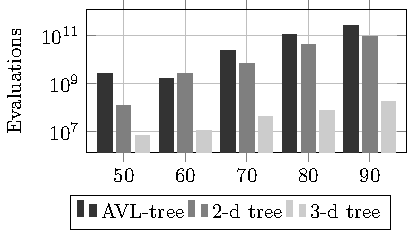
\includegraphics[scale=1.1]{tab/cmp/3dimA}
  \caption{Tipo A}
  \label{fig:sub5}
\end{subfigure}%
\begin{subfigure}{.5\textwidth}
  \centering
  %\begin{tikzpicture}
\begin{axis}[
	x tick label style={ /pgf/number format/1000 sep=},
	width=\cmpW, height=\cmpH,
	ylabel=Evaluations,
	ymode=log,
	grid = both,
	grid style={line width=.0pt, draw=gray!00},
	major grid style={line width=.2pt,draw=gray!50},
	%xlabel=Number of items (n),
	enlargelimits=0.15,
	legend style={at={(\legX,\legY)},
		anchor=north,legend columns=-1},
	ybar=2pt,% configures `bar shift'
	bar width=7pt,
	point meta=y *10^-7, % the displayed number
	cycle list = {black!80,black!50,black!20}
]

\addplot+[fill, text=black]
  coordinates {
    (100,2580591.4)
    (200,367842367.9)
    (300,7975491375.7)
    (400,72030125537.7)
  };

\addplot+[fill, text=black]
  coordinates {
    (100,1571248.6)
    (200,151476739.2)
    (300,2791493175.3)
    (400,45272872459.5)
  };
  
\addplot+[fill, text=black]
  coordinates {
    (100,912878.0)
    (200,29237583.4)
    (300,226471349.8)
    (400,960366212.0)
  };

\legend {AVL-tree,\dtree{2}, \dtree{3}}
\end{axis}
\end{tikzpicture}
  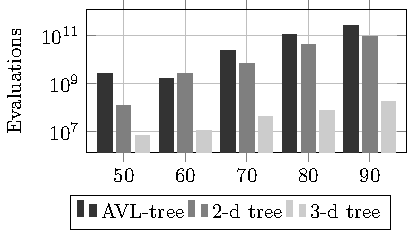
\includegraphics[scale=1.1]{tab/cmp/3dimA}
  \caption{Tipo B}
  \label{fig:sub6}
\end{subfigure}
\begin{subfigure}{.49\textwidth}
  \centering
  %\begin{tikzpicture}
\begin{axis}[
	x tick label style={ /pgf/number format/1000 sep=},
	width=\cmpW, height=\cmpH,
	ylabel=Avaliações,
	ymode=log,
	grid = both,
	grid style={line width=.1pt, draw=gray!00},
	major grid style={line width=.2pt,draw=gray!50},
	%xlabel=Number of items (n),
	enlargelimits=0.15,
	xtick={20, 30, 40},
	xticklabels={20, 30, 40},
	xmin=18,
	xmax=42,
	legend style={at={(\legX,\legY)},
		anchor=north,legend columns=-1},
	ybar=2pt,% configures `bar shift'
	bar width=7pt,
	point meta=y *10^-7, % the displayed number
	cycle list = {black!80,black!50,black!20}
]

\addplot+[fill, text=black]
  coordinates {
    ( 20,221956989)
    ( 30,10861341339)
    ( 40,26505319423)
  };

\addplot+[fill, text=black]
  coordinates {
    ( 20,235426288)
    ( 30,1340276850)
    ( 40,5943925097)
  };
  
\addplot+[fill, text=black]
  coordinates {
    ( 20,1919561)
    ( 30,10225751)
    ( 40,63529280)
  };

\legend {AVL-tree,\dtree{2}, \dtree{3}}
\end{axis}
\end{tikzpicture}

  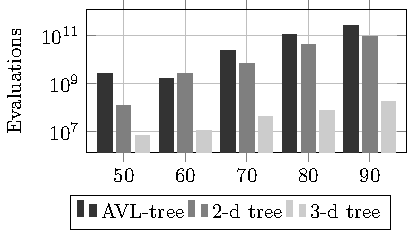
\includegraphics[scale=1.1]{tab/cmp/3dimA}
  \caption{Tipo C}
  \label{fig:sub7}
\end{subfigure}
\begin{subfigure}{.49\textwidth}
  \centering
  %\begin{tikzpicture}
\begin{axis}[
	x tick label style={ /pgf/number format/1000 sep=},
	width=\cmpW, height=\cmpH,
	ylabel=Evaluations,
	ymode=log,
	grid = both,
	grid style={line width=.0pt, draw=gray!00},
	major grid style={line width=.2pt,draw=gray!50},
	%xlabel=Number of items (n),
	enlargelimits=0.15,
	xtick={20, 30},
	xmin=17,
	xmax=33,
	legend style={at={(\legX,\legY)},
		anchor=north,legend columns=-1},
	ybar=2pt,% configures `bar shift'
	bar width=8pt,
	point meta=y *10^-7, % the displayed number
	cycle list = {black!80,black!50,black!20}
]

\addplot+[fill, text=black]
  coordinates {
    (20,481435295.3)
    (30,89269703684.8)
  };

\addplot+[fill, text=black]
  coordinates {
    (20,161607530.0)
    (30,32867842298.12)
  };
  
\addplot+[fill, text=black]
  coordinates {
    (20,2127432.7)
    (30,59136651.9)
  };

\legend {AVL-tree,\dtree{2}, \dtree{3}}
\end{axis}
\end{tikzpicture}
  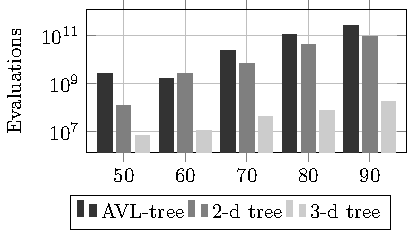
\includegraphics[scale=1.1]{tab/cmp/3dimA}
  \caption{Tipo D}
  \label{fig:sub8}
\end{subfigure}

  \caption{Número de avaliações médio do algoritmo Bazgan para instâncias 3-objetivo.}
  \label{fig:cmp3dim}
\end{figure}

É possível notar, segundo a Figura~\ref{fig:cmp3dim}, uma
leve redução no número de avaliações de solução na maioria dos casos quando
utilizada a \dtree{2} e também uma drástica redução no número de avaliações
quando utilizada a \dtree{3}, o que explica o speedup alcançado.
O resultado se deve à capacidade de indexação da \dtree{3}, a qual
indexa informação de todos os 3 valores de objetivo.
O speedup foi também possível devido ao tamanho dos conjuntos Pareto,
cuja média chegou a alcançar $8834$ (Tipo D).
Assim como no caso bi-objetivo, a baixa performance da \kdtree{} para
instâncias do tipo B, tanto no tempo computacional quanto no número de avaliações de solução,
se dá pelo reduzido tamanho dos conjuntos Pareto, tornando não proveitosa
a utilização da \kdtree{}.

Convém observar que o tamanho das instâncias utilizadas nos testes
é bem menor que a das instâncias reportadas pelo artigo original.
Isto se deu pelo alto tempo computacional demandado pela implementação
elaborada para este trabalho, cujo motivo ainda é desconhecido.
O fato, porém, não afeta as conclusões quanto à aplicação da proposta,
especialmente devido à análise do número de avaliações, sendo esta independente
do tempo computacional demandado.

\missingf{Retirei: 
``A implementação utilizada no artigo original do algoritmo Bazgan foi solicitada
aos autores, porém não houve resposta.''. Não cabe no texto da tese

\resp Ok.}

\section{Contexto Heurístico - Algoritmo SCE}

Para o contexto heurístico foram utilizadas o conjunto de instâncias propostas
e divulgadas por Zitzler e Thiele~\cite{zitzler1998multiobjective} e utilizadas desde então
pela literatura para testar a performance de heurísticas para o MOKPP~\cite{zitzler2001spea2,deb2002fast, zhang2007moea, zouache2018cooperative}.
O conjunto é composto por 6 instâncias com valores de $n$ sendo 250, 500 e 750 e
$\np$ sendo 2 e 3, uma instância para cada caso.

Com o objetivo inicial de verificar a qualidade da heurística SCE proposta para o MOKP,
foi realizado um teste inicial, comparando a qualidade das soluções geradas pela heurística
com a qualidade das soluções geradas por outros algoritmos da literatura.
Os algoritmos utilizados na comparação foram o SPEA-II~\cite{zitzler2001spea2},
NSGA-II~\cite{deb2002fast}, MOEA/D~\cite{zhang2007moea} e MOFPA~\cite{zouache2018cooperative}.
As soluções geradas por estes algoritmo, bem como as instâncias, foram
cedidas por Zouache via comunicação particular.
Para cada instância, cada um dos algoritmos foi executado 30 vezes, cada uma utilizando
uma sequência aleatória diferente, conforme praticado pela literatura.

Os parâmetros utilizados no algoritmo SCE foram os propostos pelo autor da meta-heurística
sendo apresentados na Tabela~\ref{tab:params}.
Diferentes combinações de valores de parâmetros próximos aos sugeridos foram testados
porém nenhum apresentou melhoria considerável.

\begin{table}[]
  \centering
  \begin{tabular}{c|r|p{65mm}}
\hline
  Parâmetro
   & Valor
   & \multicolumn{1}{c}{Descrição} \\ \hline
  N  &  30    & Número de complexos \\ \hline
  M  &  30    & Número de indivíduos em cada complexo\\ \hline
  P  &   5    & Número de indivíduos em cada subcomplexo\\ \hline
  K  & 400    & Número de iterações\\ \hline
  K' &  30    & Número de iterações aplicados a cada evolução de complexo\\ \hline
  c  & $n/20$ & Número de genes carregados no procedimento de cruzamento\\ \hline
\end{tabular}

  \caption{Valores de parâmetros utilizados no algoritmo SCE.}
  \label{tab:params}
\end{table}

A métrica de qualidade utilizada neste caso foi o hiper-volume do conjunto Pareto
aproximado~\cite{fonseca2006improved},
por ser considerado pela literatura~\cite{schutze2016hypervolume,beume2007sms}
a métrica mais representativa para a avaliar a qualidade do \paretoset{},
uma vez que ``a velocidade de convergência da taxa de aproximação alcançada
ao maximizar o hyper-volume é assintoticamente ótima''
conforme apresentado por Bringmann e Friedrich em~\cite{bringmann2010maximum}.
A métrica mede o hiper-volume da região contida pelos valores de objetivo das soluções.
A Figura~\ref{img:hvol2} apresenta um conjunto Pareto com 3 soluções para um problema 
bi-objetivo, cujo hiper-volume (unidades de área) é 18.
No caso de um problema 3-objetivo, o hiper-volume seria unidades de volume e assim sucessivamente.
Outras métricas como distância geracional invertida~\cite{van1998multiobjective},
cobertura de conjunto~\cite{zitzler1998multiobjective}
e espaçamento de solução~\cite{schott1995fault} são válidas para evidenciar
aspectos específicos do \paretoset{}, o que não é o objetivo do presente trabalho.

\missingf{A justificativa de  uso do hiper-volume quanto comparada as alternativas está meio fraco. Porque é bastante representativa e suficiente?
Quais as evidencias quantitativas que tem para isso? Tem como melhorar?

\resp O hyper-volume é a métrica ``padrão'' para medir qualidade de \paretoset{}.
Como o objetivo do experimento é apenas validar a heurística diante das outras,
não achei proveitoso apresentar as outras métricas.

Reestruturei o texto, citando dois artigos que comentam a importância do hiper-volume e um trabalho que prova que o hiper-volume
é a que melhor expressa a aproximação do \paretoset{} do valor ótimo.
}

\begin{figure}
  \centering
  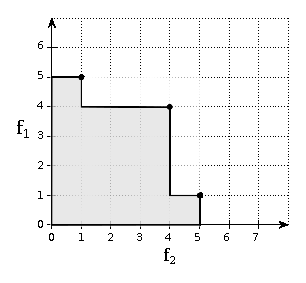
\includegraphics[width=0.3\textwidth]{img/sce/hypervol2}
  \caption{Exemplo de conjunto Pareto bi-objetivo possuindo 18 unidades hiper-volume (área).}
  \label{img:hvol2}
\end{figure}

Visando validar a qualidade do algoritmo SCE, a Tabela~\ref{tab:zitzler} apresenta os
resultados alcançados pelas heurísticas expressos em porcentagem média de hiper
volume alcançado, em relação ao maior hiper-volume de solução conhecida para a instância.
Cada célula apresenta a média de 30 execuções.
Em destaque estão os melhores valores de hiper-volume.
\begin{table}[]
  \centering
  \begin{tabular}{cc|c|c|c|c|c}
  \hline
  { m} &
  { n} &
  { SPEA2} &
  { NSGA-II} &
  { MOEA/D} &
  { MOFPA} &
  { SCE} \\ \hline
  \multirow{2}{*}{2} & { 250} & 90.4 & 86.3 & 96.9 & \textbf{97.8} & 93.6 \\ \cline{2-7}
   & { 500} & 87.6 & 81.7 & 96.9 & \textbf{97.8} & 92.7 \\ \cline{2-7}
   & { 750} & 85.9 & 79.2 & 98.4 & \textbf{99.2} & 92.3 \\ \hline
  \multirow{2}{*}{3} & { 250} & 83.3 & 77.4 & 99.0 & \textbf{99.7} & 89.4 \\ \cline{2-7}
   & { 500} & 72.8 & 65.9 & 92.9 & \textbf{93.6} & 79.4 \\ \cline{2-7}
   & { 750} & 77.5 & 73.3 & 94.7 & \textbf{95.2} & 79.8 \\ \hline
\end{tabular}

  \caption{Hiper-volume médio alcançado por cada heurística.}
  \label{tab:zitzler}
\end{table}

Pode-se observar pela Tabela~\ref{tab:zitzler} que, apesar de não apresentar resultados
melhores que os do MOEA/D e que os do recente MOFPA,
os resultados alcançados pelo SCE foram consistentes,
sendo melhores que as heurísticas SPEA2 e NSGA-II.

\missingf{Tem que aprofundar essa discussão: porque o SCE foi superior e inferior a cada metaheuristica? Será que as melhores usam mais conhecimento especifico do problema do que as outras?

\resp 
Nenhuma delas usa conhecimento específico. Aliás, o NSGA-II, o SPEA-II e o MOEA/D são heurísticas genéricas.
Apenas a proposta do MOFPA foi dedicada ao MOKP, ainda assim não utiliza nenhum conhecimento específico, é só uma proposta de PSO+Firefly
que testaram no MOKP.
Nem no artigo do MOFPA encontrei alguma indicação de porque ficou melhor que as outras.
Seria mesmo interessante explicar por que são melhores, mas estou achando difícil. Não sei o que dizer.
}

A utilização da \kdtree{} foi comparada à utilização da lista encadeada,
por ser a estrutura utilizadas nos algoritmos heurísticos em questão.
A Tabela~\ref{tab:scecpu} apresenta o tempo computacional médio demandado pela execução do
algoritmo SCE para cada uma das 6 instâncias para a utilização da Lista encadeada,
\dtree{2} e, no caso 3-objetivo, \dtree{3}.
A coluna $\ndcol$ apresenta o tamanho médio do conjunto Pareto aproximado dado como
resposta pelo algoritmo.

\missingf{Porque usou lista e nao avl? No exato usou AVL. Porque mudou? Tem que justificar.

\resp Como o objetivo dos testes era comparar a utilização da \kdtree{} com o que a literatura utiliza,
eu utilizei apenas a lista no caso heurístico.
A AVL eu só utilizei no exato por ter sido a proposta da Bazgan para o algoritmo exato.
Adicionei essa explicação ao texto.
}

\begin{table}[]
  \centering
  \begin{tabular}{crr|r|rr|rr}
  \hline
  %%%%%%%%%%%%%%%%%
  %   HEADER
  %%%%%%%%%%%%%%%%%
  \multicolumn{3}{c|}{Instância}
  & \multicolumn{1}{c|}{Lista}
  & \multicolumn{2}{c|}{\dtree{2}}
  & \multicolumn{2}{c}{\dtree{3}}
    \\
  $\np$
  & $n$ \phantom{a}
  & $\ndcol$
  & tempo (s)
  & tempo (s)
  & speedup
  & tempo (s)
  & speedup
    \\ \hline
\multirow{2}{*}{2}
 & 250 &  88.4 & \textbf{  9.3} & 13.1 & 0.71 & -- & -- \\ \cline{2-8}
 & 500 & 106.0 & \textbf{ 14.3} & 18.3 & 0.78 & -- & -- \\ \cline{2-8}
 & 750 & 120.4 & \textbf{ 18.7} & 22.3 & 0.84 & -- & -- \\ \hline
\multirow{2}{*}{3}
 & 250 & 705.5 &  9.8   & 10.1 & 0.97 & \textbf{  9.1} & 1.08 \\ \cline{2-8}
 & 500 & 672.8 & 15.6   & 16.0 & 0.98 & \textbf{ 15.2} & 1.03 \\ \cline{2-8}
 & 750 & 646.0 & 22.0   & 24.2 & 0.91 & \textbf{ 21.8} & 1.01 \\ \hline
\end{tabular}

  \caption{Tempo computacional médio do algoritmo SCE para instâncias Zouache.}
  \label{tab:scecpu}
\end{table}

A Figura~\ref{fig:cmpsce} apresenta o número médio de avaliações de solução
para os casos (a) bi-objetivo e (b) 3-objetivo.
O eixo horizontal refere-se ao tamanho da instância (número de itens)
enquanto que o eixo vertical refere-se ao número médio de avaliações de solução.

\missingf{Vc usou várias vezes "numero medio de avaliação de soluções" e agora usou "numero medio de avaliações de solução". 
Favor uniformizar ao longo do texto do capítulo. Eu prefiro "numero medio de avaliações de solução"

\resp Ok. Uniformizei assim.}

\begin{figure}
\centering
\begin{subfigure}{.5\textwidth}
  \centering
  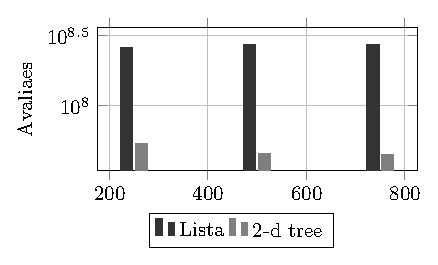
\includegraphics[scale=1.1]{tab/sce/cmpres2}
  \caption{Instâncias 2-objetivo}
  \label{fig:cmpsce2}
\end{subfigure}%
\begin{subfigure}{.5\textwidth}
  \centering
  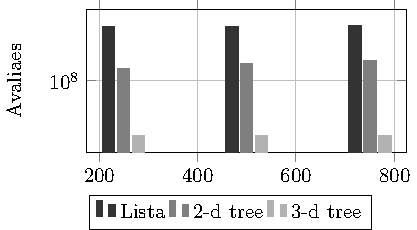
\includegraphics[scale=1.1]{tab/sce/cmpres3}
  \caption{Instâncias 3-objetivo.}
  \label{fig:cmpsce3}
\end{subfigure}
\caption{Número de avaliações médio do algoritmo SCE para instâncias Zouache.}
\label{fig:cmpsce}
\end{figure}

Pode-se observar que a \dtree{2} não foi capaz de oferecer melhoria no tempo computacional
demandado pelo algoritmo, apesar da redução no número de avaliações de solução.
Este resultado se deve ao tamanho reduzido do conjunto Pareto mantido pelo algoritmo,
em especial para os casos bi-objetivo.
Para os casos 3-objetivo ainda se pode observar um pequeno speedup no
caso da \dtree{3}, devido a se ter maiores conjuntos Pareto,
o que não torna favorável o \emph{overhead} adicional da estrutura.

\missingf{Interessante expandir mais a dicussao do porque o resultado nao foi bom!

\resp Complementei apontando o problema do overhead. (no parágrafo abaixo eu continuo a discussão) }

Vale também observar que, para o algoritmo heurístico,
a demanda de operações de verificação
de dominância é relativamente pequena em relação às outras operações relacionadas
ao caráter evolucionário do algoritmo, diferentemente do algoritmo exato,
cujo desenvolvimento se baseia em sua maioria na operação de verificação de dominância,
o que também explica o insucesso da \kdtree{} nesse caso.


% Conclusão
\chapter{Conclusão}
\section{Contribuições}

O presente trabalho propõe a indexação multidimensional das soluções
do problema da mochila multiobjetivo,
como proposta de aceleração das operações de verificação de dominância de solução.
A operação de verificação de dominância é uma das principais
operações necessárias para a resolução do problema.
A indexação multidimensional das soluções tem por objetivo
reduzir o número de avaliações de soluções necessárias para a execução da operação,
diminuindo consequentemente o tempo computacional demandado.

Há na literatura a proposta de utilização da quadtree como estrutura de dados
de indexação de soluções de problemas multiobjetivo.
Porém a estratégia mostrou-se eficaz apenas em casos bi-objetivos de conjuntos Paretos consideravelmente extensos.
Conjectura-se que essa ineficiência é decorrente
do alto \emph{overhead} da estrutura, especialmente em casos com mais de dois objetivos.

Para que a proposta de indexação fosse possível,
foi definido no presente trabalho um mapeamento entre a operação
de verificação de dominância e o problema da busca de faixa.
O problema de busca de faixa consiste em verificar a existência de pontos em uma determinada
região do espaço multidimensional.
Esse problema é bem conhecido em áreas como computação gráfica, geometria computacional e jogos,
onde a \kdtree{} é geralmente utilizada como estrutura de dados auxiliar.
Sendo assim, a proposta do presente trabalho foi a utilização da \kdtree{}
como estrutura auxiliar da operação de verificação de dominância.

A aplicação e o comportamento da \kdtree{} junto à operação
foram discutidos, bem como os da lista encadeada e da árvore AVL,
estruturas até então utilizadas pela literatura para este fim.
O desempenho da proposta de indexação foi testado no contexto exato e heurístico.

No contexto exato, a proposta foi aplicada ao algoritmo Bazgan,
considerado pela literatura como o mais eficiente atualmente para o problema da mochila multiobjetivo.
A performance do algoritmo foi comparada através de experimentos computacionais.
Para tanto, foi considerada a mesma proposta de instâncias empregada pela literatura,
sendo quatro tipos de instâncias bi-objetivo e dois tipos de instâncias 3-objetivo.
Para o caso 3-objetivo foram ainda propostas mais dois tipos de instâncias,
sendo estas generalizações de seus respectivos casos bi-objetivos.

Os resultados dos experimentos computacionais utilizando o algoritmo Bazgan,
mostraram que a proposta de indexação multidimensional possibilitou o speedup
de até $2.3$ para os casos bi-objetivo, e até $15.5$ para casos 3-objetivo.
A proposta não se mostrou eficiente apenas em instâncias consideradas fáceis,
cujos conjuntos Pareto têm tamanhos consideravelmente reduzidos em relação
às demais instâncias.
Nesses casos, onde se dá a manipulação de poucas soluções,
o \emph{overhead} computacional da \kdtree{} torna sua utilização ineficaz.

No contexto heurístico, a indexação multidimensional
foi aplicada ao algoritmo SCE para o MOKP, proposto também neste trabalho.
Primeiramente o SCE foi adaptado para resolver problemas multiobjetivo.
Para isso, a aptidão das soluções foi definida com base na ordenação
em frontes não dominados.
A aproximação do \paretoset{} foi gerada com o auxílio de um arquivo externo.
Em seguida, foi estabelecida a implementação específica para o MOKP,
definindo-se a operação de geração de solução viável
aleatória e a operação de cruzamento de soluções.

A validade da implementação do algoritmo SCE para o MOKP foi primeiramente
avaliada e comparada com os principais algoritmos da literatura,
não tendo melhores resultados que as
heurísticas de estado-da-arte, porém tendo resultados superiores aos
das heurísticas mais antigas.

Os experimentos computacionais no contexto heurístico
foram realizados sobre o conjunto de 6 instâncias,
utilizado pela literatura para avaliar a performance de heurísticas para o MOKP.
Apesar de reduzir consideravelmente o número de avaliações de soluções,
a utilização da \kdtree{} não apresentou eficiência relevante quanto ao tempo computacional
na abordagem heurística, tendo pior performance nas instâncias com \paretoset{}
relativamente pequenos.

Pode-se concluir que a utilização da \kdtree{} é capaz de reduzir consideravelmente
o número de avaliações de soluções na maioria dos casos, além de também reduzir o tempo computacional
demandado em casos em que é necessário executar a verificação de dominância em grandes
conjuntos de solução.
Os resultados evidenciam ser indispensável
a utilização de uma estrutura de indexação multidimensional,
nos casos de problemas com mais de 2 objetivos com grandes
conjuntos de solução.
Vale ressaltar que os algoritmos não foram alterados, somente
a forma de indexação das soluções, a qual pode ser aplicada a qualquer algoritmo
que faz utilização da operação de verificação de dominância de solução.

%\missingf{afirmacao forte: "Segundo os resultados, a utilização de uma estrutura de indexação multidimensional
%mostra-se indispensável no caso de problemas com mais de 2 objetivos com grandes
%conjuntos de solução." em vez de mostra, alterei para evidencia... 
%
%\resp Ok. Melhor.}

Notou-se porém, que em casos onde o número de soluções manipuladas é pequeno, a utilização
da \kdtree{} não é recomendável, pois apesar de apresentar redução no número de
avaliações, o \emph{overhead} da estrutura dificulta uma redução no tempo computacional demandado.

\section{Trabalhos Futuros}

Como trabalho futuro pretende-se verificar a performance da \kdtree{} em outros problemas
multiobjetivos, uma vez que o crescimento do \paretoset{} não é
uma característica específica do problema em questão, mas observado
em problemas multiobjetivo de forma geral, visto que as possibilidades de soluções
eficientes aumentando dado o tamanho da instância,
especialmente para casos com mais dois objetivos~\cite{ehrgott2013multicriteria}.

Outro ponto a ser explorado é a consideração de outras estruturas de dados
para auxílio à operação de verificação de dominância.
Uma das estruturas a ser considerada é a ND-Tree, proposta
em~\cite{jaszkiewicz2017} como estrutura de dados para auxiliar
a operação de verificação de dominância.
Vale também considerar a proposta de uma estrutura dedicada ao
problema de verificação de dominância, considerando que as
soluções pertencentes a um \paretoset{} possuem uma distribuição espacial
característica, na qual nenhuma é dominada por outra.

Pretende-se também aprimorar a implementação do SCE para o MOKP.
Uma possibilidade seria o aperfeiçoamento das soluções
através da utilização de conhecimentos específicos do problema.
Outra possibilidade seria realizando um pré-processamento sobre o problema inicial,
transformando-o em um problema mais simples ou dividindo-o em sub-problemas
menores.

Além das propostas de contribuição, pretende-se investigar a causa da
presente implementação do algoritmo Bazgan demandar mais tempo computacional
que o relatado pela literatura.


\missingf{Sugiro expandir a discussão de trabalhos futuros}

\missingf{ na verdade acho que a Conclusao tem que ser expandida como um todo. Tá parecendo conclusao de artigo, que tem limitacao de espaço. Vc poderia falar mais de cada um dos itens comentados, até apresentar exemplos para esclarecer os leitores.}


\postextual

\bibliography{tex/references}

\end{document}
